\section{Konzept}
\label{sec:TeilB_Konzept}
Um die Entwicklung zielführend zu gestalten ist neben der Bauteilrecherche eine grobe Hardwarearchitektur zu erstellen, welche sich zunehmend verfeinert. Die letztendliche Architektur wird als Ausgangspunkt für weitere Entwicklungen genommen. Treten Probleme während der Entwicklung auf, wie z. B. Bauteile sind nicht lieferbar, zu teuer oder die gewünschten Bauformen nicht verfügbar, sind Alternativen zu finden. Dabei steht im Mittelpunkt das Konzept bestenfalls nur minimal ändern zu müssen. Um solchen Probleme zu vermeiden, ist es sinnvoll ein vollständiges Konzept, sowie eine Bauteildatenbank inklusive Lieferdaten der Bauteile im Vorfeld zu erstellen. Das Projekt orientiert sich bezüglich der Konversion von HDMI nach RGB und LVDS an der Application Note SLLA325A von Texas Instruments (siehe \cite{TI2011}).
\begin{figure}[htp]
%\begin{minipage}[t]{0.8\textwidth}
%\begin{figure}[h]
	\centering
\fbox{	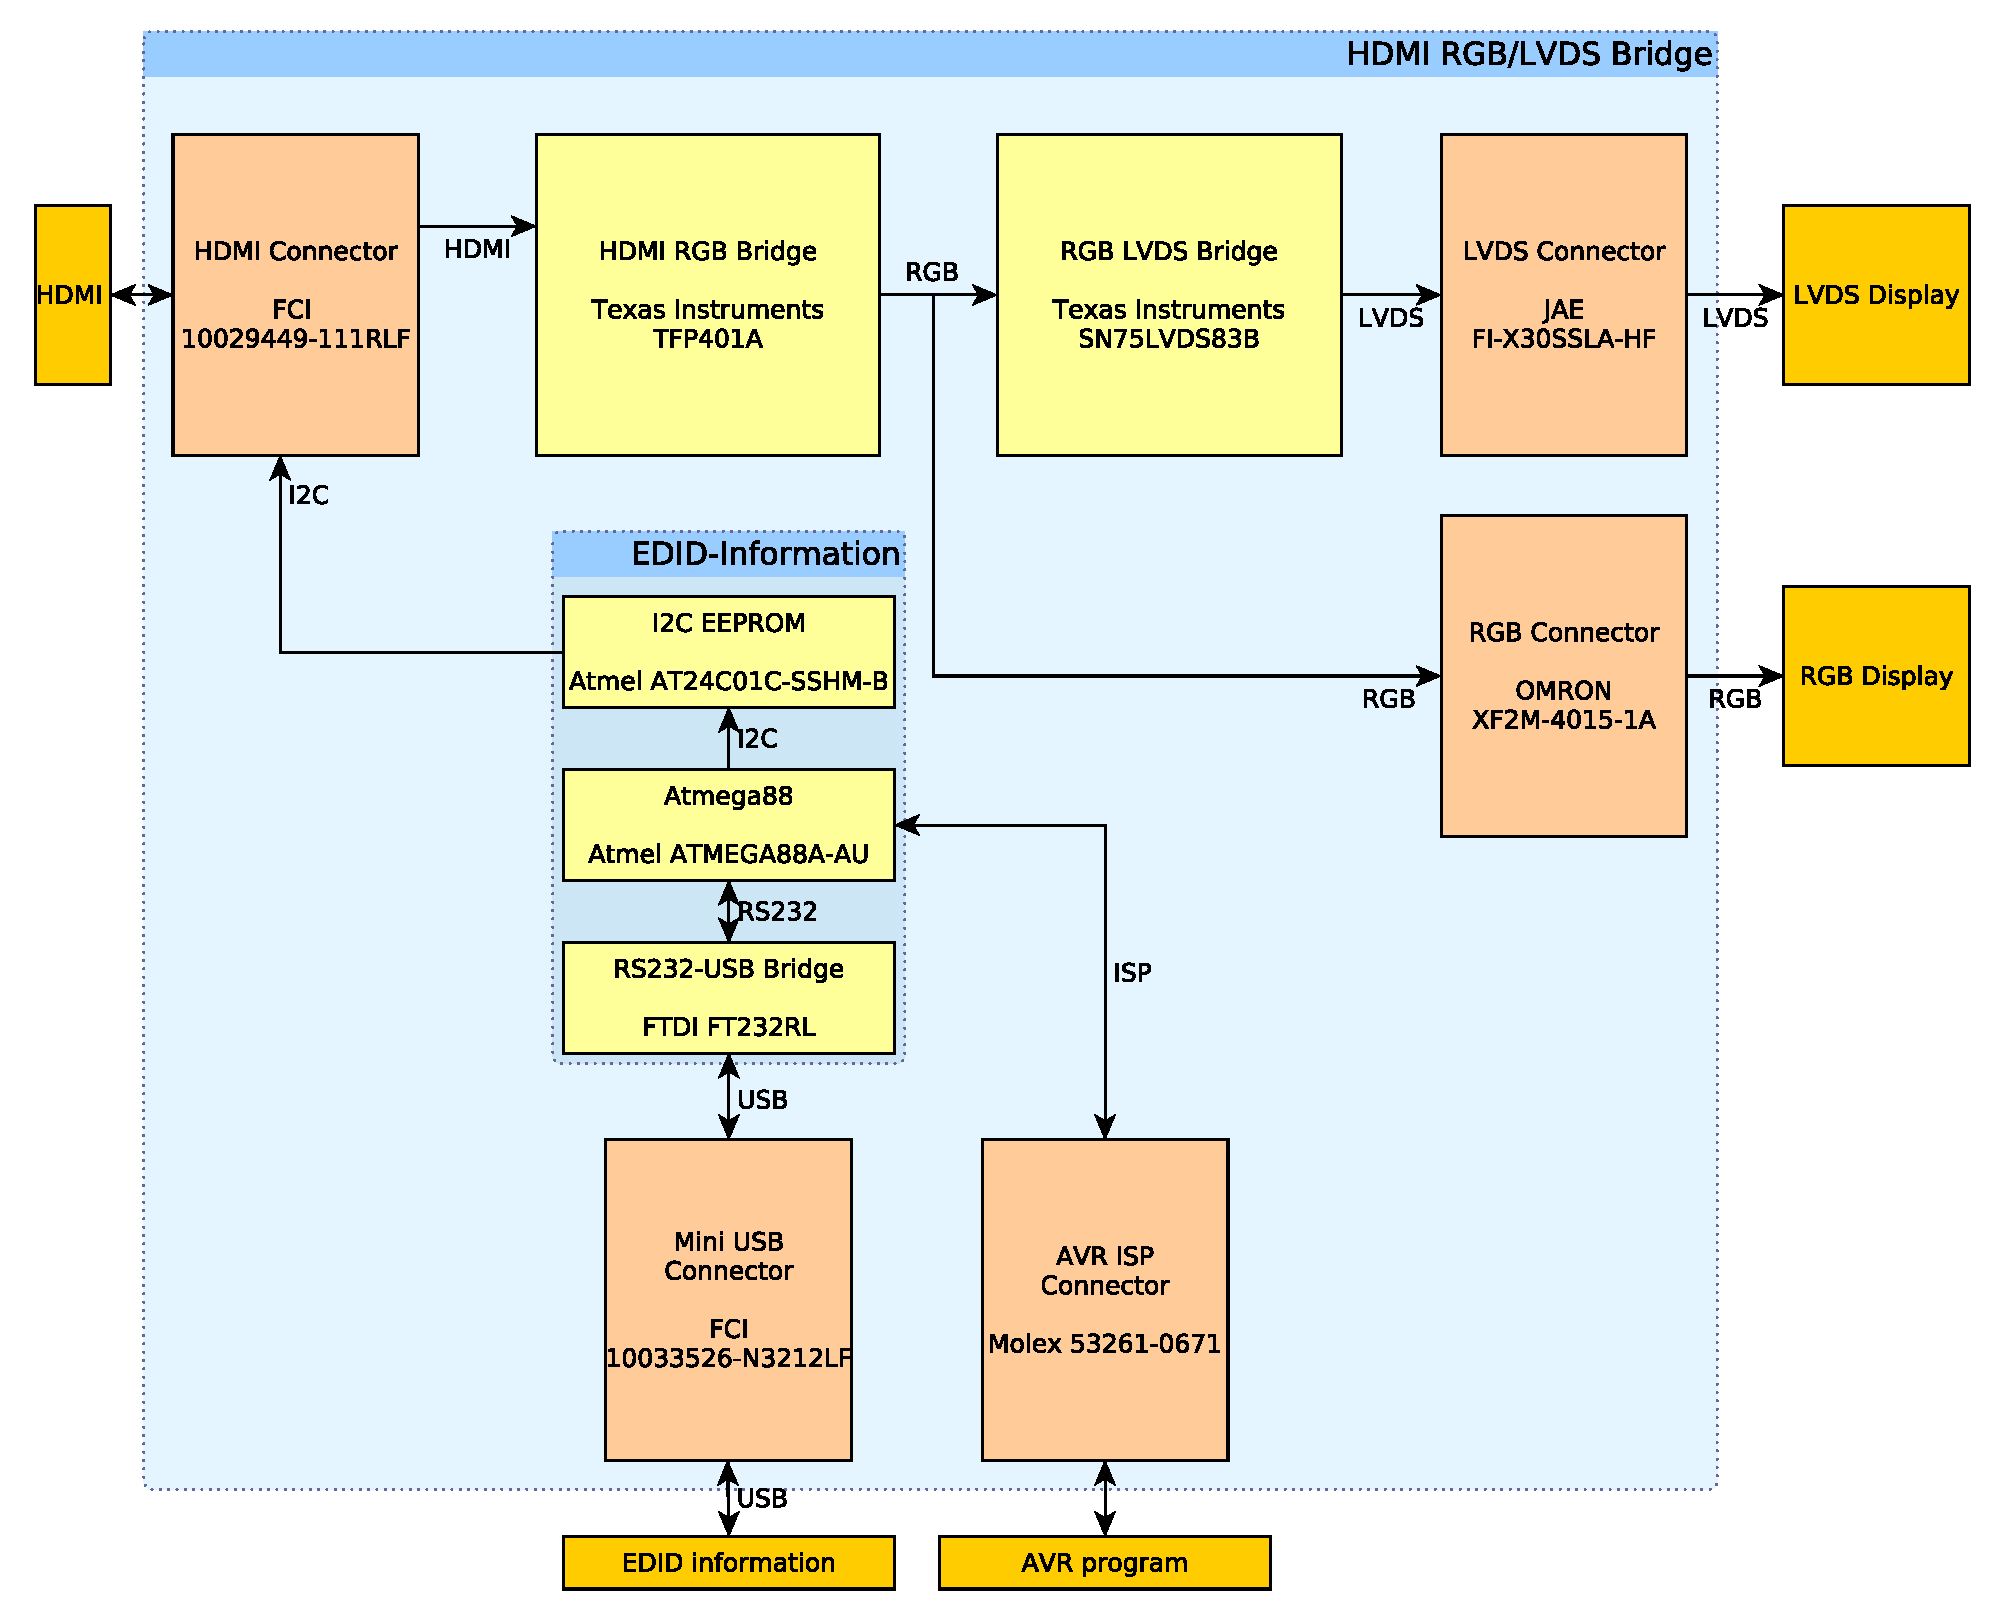
\includegraphics[width=1.0\textwidth]{TeilB/Architektur.pdf}}
	\caption{Hardware-Architektur}
	\label{fig:teilb_architektur}
\end{figure}

\refa{fig:teilb_architektur} zeigt die komplette Architektur des Projekts mit allen notwendigen Eckpunkten und Verbindungen. So sind Schnittstellen nach außen mit rot und die interne Logik mit gelb markiert. Als Signalquelle wird das HDMI-Signal eingespeist und in die \code{HDMI-RGB-Bridge} geleitet. Der Baustein \code{TFP401A} konvertiert die eingehenden HDMI-Signale zum RGB-Bus. Hier kann direkt über einen FPC-Stecker\footnote{FPC: Fine Pitch Connector} ein RGB-Display anschlossen werden. Die Leitungen werden zu einer RGB-LVDS-Bridge weitergeleitet. Diese wandelt die RGB-Signale in LVDS-Signale entsprechend der benötigten Beschaltung des verwendeten Displays um. Wird die Platine mit einer Quelle verbunden, so tauschen beide Informationen aus. Dabei ließt die Quelle Leistungsdaten bzgl. Auflösung, Timings, etc. aus einem EEPROM  im Anzeigegerät aus. Diese Daten werden als EDID-Daten\footnote{EDID: Extended Display Identification Data} bezeichnet (siehe \cite{edid2000}). Gespeichert werden die EDID-Daten üblicherweise in einem EEPROM\footnote{EEPROM: Electrically Eraseable Programmable Read-Only Memory}, auf welches mit dem $I^2C$-Bus zugegriffen wird. Um das EEPROM mit korrekten Inhalten beschreiben zu können, ist eine Baugruppe mit den Namen \code{EDID-Information} realisiert (siehe \refa{fig:teilb_architektur}). Der verwendete USB-Seriell-Konverter FT232RL kommuniziert mit einem 8-Bit Atmel ATMega88 Prozessor, welcher das $I^2C$-EEPROM direkt beschreiben kann. Um die korrekten EDID-Informationen in das EEPROM zu schreiben ist die zugehörige PC Software zu verwenden (siehe \refc{edid_pc}).\newpage